%----------------------------------------------------------------------------------------
%	PACKAGES AND OTHER DOCUMENT CONFIGURATIONS
%----------------------------------------------------------------------------------------
\documentclass[12pt]{article}
\usepackage{graphicx}
\usepackage{amsmath,amsfonts,stmaryrd,amssymb} % Math packages
\usepackage{bm}
\usepackage{steinmetz}
\usepackage{enumitem}
\graphicspath{{images/}}
\usepackage{float}
\usepackage{cancel}
\usepackage{hyperref}
\hypersetup{
	colorlinks=true,
	linkcolor=blue,
	filecolor=magenta,      
	urlcolor=cyan,
	pdftitle={Overleaf Example},
	pdfpagemode=FullScreen,
}
\urlstyle{same}
\usepackage{mathtools}
\usepackage{fancyhdr}
\usepackage{xcolor}
\usepackage[american,RPvoltages]{circuiTikz}
\usepackage{tikz, tikz-cd}
\usepackage{pgfplots}
\usepackage{siunitx}
\usetikzlibrary{spy,shapes,arrows, arrows.meta, bending, decorations.markings}
\pgfplotsset{width=10cm,compat=1.18}
\usepackage{lmodern} % package for changing font size
\usepackage{lastpage}
\renewcommand{\figurename}{Figura}
\usepackage{tcolorbox}
\usepackage{lipsum}
%\usepackage{enumerate} % Custom item numbers for enumerations
\usepackage[ruled]{algorithm2e} % Algorithms
\usepackage[framemethod=tikz]{mdframed} % Allows defining custom boxed/framed environments
\usepackage{listings} % File listings, with syntax highlighting
%\lstset{basicstyle=\ttfamily,} % Typeset listings in monospace font
\usepackage{lipsum}
\tcbuselibrary{listings,theorems,skins,vignette,raster,breakable,magazine,poster,fitting,hooks}
\usepackage[T1]{fontenc}
\usepackage{tgbonum}
 \fontfamily{garamond}
\definecolor{myblue}{RGB}{24, 51, 73}
%----------------------------------------------------------------------------------------
%	DOCUMENT MARGINS
%----------------------------------------------------------------------------------------

\usepackage{geometry} % Required for adjusting page dimensions and margins
\geometry{
	paper=a4paper, % Paper size, change to letterpaper for US letter size
	top=2.5cm, % Top margin
	bottom=3cm, % Bottom margin
	left=2cm, % Left margin
	right=2.5cm, % Right margin
	headheight=14pt, % Header height
	footskip=1.5cm, % Space from the bottom margin to the baseline of the footer
	headsep=1.2cm, % Space from the top margin to the baseline of the header
	%showframe, % Uncomment to show how the type block is set on the page
}

%----------------------------------------------------------------------------------------
%	FONTS
%----------------------------------------------------------------------------------------

\usepackage[utf8]{inputenc} % Required for inputting international characters
\usepackage[T1]{fontenc} % Output font encoding for international characters
\usepackage{XCharter} % Use the XCharter fonts
\usepackage{tgbonum}

\makeatletter
\pgfcircdeclarebipole{}{\ctikzvalof{bipoles/vsourcesin/height}}{sVpm}{\ctikzvalof{bipoles/vsourcesin/height}}{\ctikzvalof{bipoles/vsourcesin/width}}{
	
	\pgfsetlinewidth{\pgfkeysvalueof{/tikz/circuitikz/bipoles/thickness}\pgfstartlinewidth}
	\pgfpathellipse{\pgfpointorigin}{\pgfpoint{0}{\pgf@circ@res@up}}{\pgfpoint{\pgf@circ@res@left}{0}}
	\pgfusepath{draw}     
	\pgftext[bottom,rotate=90,y=\ctikzvalof{bipoles/vsourceam/margin}\pgf@circ@res@down]{\scriptsize$-$}
	\pgftext[top,rotate=90,y=\ctikzvalof{bipoles/vsourceam/margin}\pgf@circ@res@up]{\scriptsize$+$}
	
	\pgf@circ@res@up = .35\pgf@circ@res@up
	\pgfscope
	\pgftransformrotate{90}
	\pgfpathmoveto{\pgfpoint{-\pgf@circ@res@up}{0cm}}
	\pgfpathsine{\pgfpoint{.5\pgf@circ@res@up}{.4\pgf@circ@res@up}}
	\pgfpathcosine{\pgfpoint{.5\pgf@circ@res@up}{-.4\pgf@circ@res@up}}
	\pgfpathsine{\pgfpoint{.5\pgf@circ@res@up}{-.4\pgf@circ@res@up}}
	\pgfpathcosine{\pgfpoint{.5\pgf@circ@res@up}{.4\pgf@circ@res@up}}
	\pgfusepath{draw}
	\endpgfscope
}
\def\pgf@circ@sVpm@path#1{\pgf@circ@bipole@path{sVpm}{#1}}
\compattikzset{sinusoidal voltage source pm/.style = {\circuitikzbasekey, /tikz/to path=\pgf@circ@sVpm@path, \circuitikzbasekey/bipole/is voltage=true, \circuitikzbasekey/bipole/is voltageoutsideofsymbol=true, v=#1 }}
\compattikzset{sVpm/.style = {\comnpatname sinusoidal voltage source pm = #1}}

\pgfcircdeclarebipole{}{\ctikzvalof{bipoles/vsourcesin/height}}{sVpmh}{\ctikzvalof{bipoles/vsourcesin/height}}{\ctikzvalof{bipoles/vsourcesin/width}}{
	
	\pgfsetlinewidth{\pgfkeysvalueof{/tikz/circuitikz/bipoles/thickness}\pgfstartlinewidth}
	\pgfpathellipse{\pgfpointorigin}{\pgfpoint{0}{\pgf@circ@res@up}}{\pgfpoint{\pgf@circ@res@left}{0}}
	\pgfusepath{draw}     
	\pgftext[center,x=0.2\pgf@circ@res@down-\ctikzvalof{bipoles/vsourceam/margin}\pgf@circ@res@down]{\scriptsize$-$}
	\pgftext[top,rotate=90,y=\ctikzvalof{bipoles/vsourceam/margin}\pgf@circ@res@up]{\scriptsize$+$}
	
	\pgf@circ@res@up = .35\pgf@circ@res@up
	\pgfscope
	\pgftransformrotate{90}
	\pgfpathmoveto{\pgfpoint{-\pgf@circ@res@up}{0cm}}
	\pgfpathsine{\pgfpoint{.5\pgf@circ@res@up}{.4\pgf@circ@res@up}}
	\pgfpathcosine{\pgfpoint{.5\pgf@circ@res@up}{-.4\pgf@circ@res@up}}
	\pgfpathsine{\pgfpoint{.5\pgf@circ@res@up}{-.4\pgf@circ@res@up}}
	\pgfpathcosine{\pgfpoint{.5\pgf@circ@res@up}{.4\pgf@circ@res@up}}
	\pgfusepath{draw}
	\endpgfscope
}
\def\pgf@circ@sVpmh@path#1{\pgf@circ@bipole@path{sVpmh}{#1}}
\compattikzset{sinusoidal voltage source pmh/.style = {\circuitikzbasekey, /tikz/to path=\pgf@circ@sVpmh@path, \circuitikzbasekey/bipole/is voltage=true, \circuitikzbasekey/bipole/is voltageoutsideofsymbol=true, v=#1 }}
\compattikzset{sVpmh/.style = {\comnpatname sinusoidal voltage source pmh = #1}}
\makeatother


%----------------------------------------------------------------------------------------
%	BEGIN DOCUMENT
%----------------------------------------------------------------------------------------

\begin{document}
	%\thispagestyle{empty}
	\begin{tikzpicture}[remember picture, overlay]
		\node[anchor=north west, inner sep=0pt] at (current page.north west) {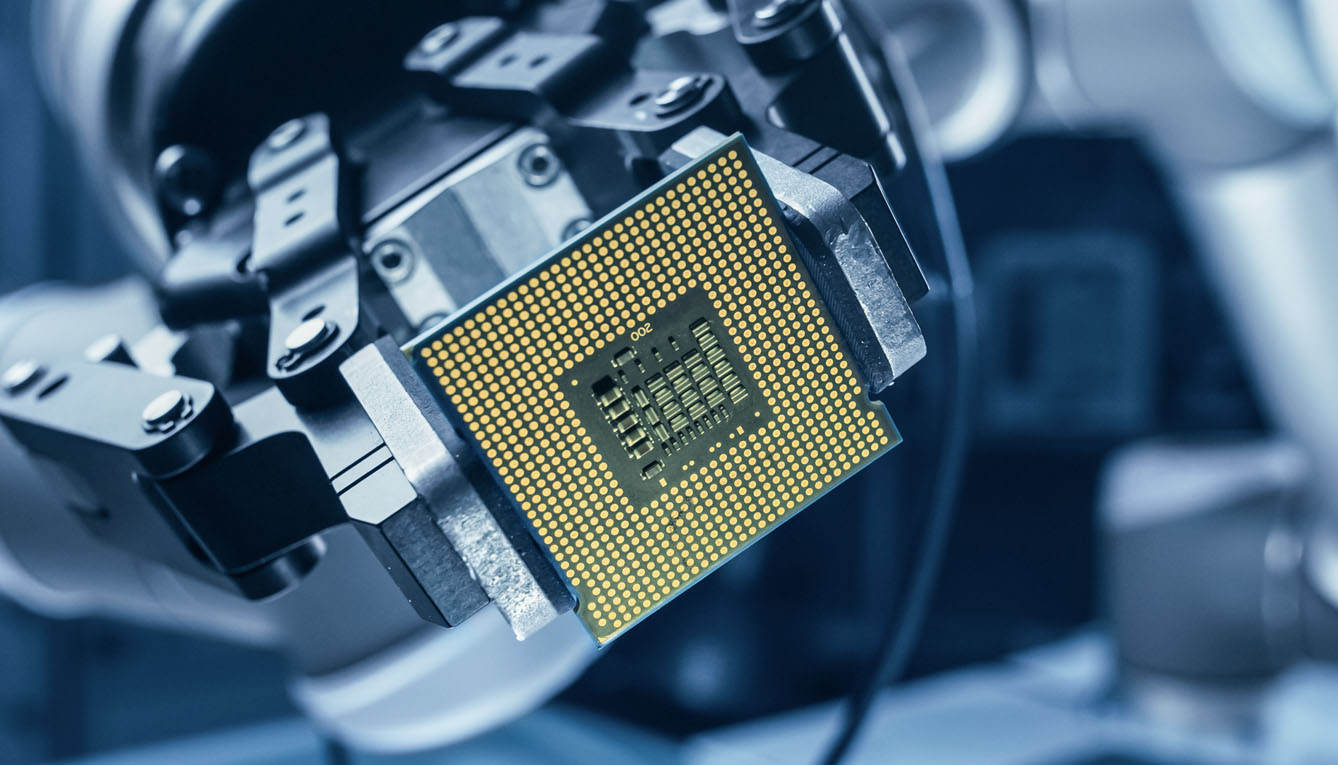
\includegraphics[width=\paperwidth, height=.5\paperheight]{picture1}};
	\end{tikzpicture}

	\vspace{13cm}
	\noindent \textcolor{myblue}{\fontsize{40pt}{40pt}\selectfont \textbf{Simulador de Inductancia}}\\\\
	{\fontsize{18pt}{18pt}\selectfont Julio, 2023} 
	
	\newpage
	\section*{Fundamentos de STM32 - Timers e Interrupciones}
	Los timers son una de las características más importantes en los micocontrtoladores modernos
	
	\subsection*{Inductor simulado de Riordan}
	\begin{figure}[H]
		\centering	
		\begin{tikzpicture}[]
			\ctikzset{resistor = european}
			%\draw[step=.5, gray,very thin] (-6.4,-6.4) grid (8.4,8.4);
			\draw (0,0)  node[op amp, noinv input up, anchor=+](OA){\texttt{OA1}};
			\draw (OA.+) to[short, -*] ++(-1,0) coordinate(nodeA) to[short, f_<=$I(s)$, -o] ++(-3,0) node[left]{$E(s)$} coordinate(point+);
			\draw (OA.-) to[short] ++(-1,0)
						 to[short, -*] ++(0,-2) coordinate(nodeB) node[left]{$V_m$};
			\draw (nodeB) to[R, l=$Z_2$] (nodeB -| OA.out) -- (OA.out);
			\draw (nodeB) to[R, l=$Z_1$, -*] ++(0,-3) coordinate(nodeG) node[ground]{};
			\draw (nodeG) to[short, -o] ++(-3,0) coordinate(point-);
			\coordinate (M) at ($(point+)!0.5!(point-)$);
			\draw  [cyan, ->] (M) node[cyan,left]{$Z_{IN}(s)$} -- ++(1,0) ;
			\draw (OA.out) ++(4.5,0.98) node[op amp, noinv input up, anchor=+](OA2){\texttt{OA2}};
			\draw (OA.out) to[R, l=$Z_3$, *-*] ++(3.5,0) coordinate(nodeF)
						to[short] ++(1,0);
			\draw (nodeF) node[above]{$V_n$};
			\draw (nodeF) to[short] ++(0,-2) coordinate(nodeE)
						  to[R, l=$Z_4$] (nodeE -| OA2.out) -- (OA2.out);
			\draw (OA2.+) to[short] ++(-1,0)
						  to[short, -*] ++(0,2) coordinate(nodeH);
			\draw (nodeH) to[R, l=$Z_5$] (nodeH -| OA2.out) -- (OA2.out);
			\draw (OA2.out) to[short, *-] (OA2.out);
			\draw (nodeH) to[short] (nodeH -| nodeA) -- (nodeA);
			\draw (OA.out) node[above]{$V_1$};
			\draw (OA2.out) node[right]{$V_2$};
		\end{tikzpicture}
		\caption{Amplificador Diferencial.}	
		\label{fig:figura1}
	\end{figure}
	
	\noindent El amplificador OA1 se trata de un amplificador no inversor, por lo tanto, el voltaje en el nodo $V_1$ es
	\begin{align}
		V_1(s) = \frac{Z_1(s) + Z_2(s)}{Z_1(s)}E(s)
	\end{align}
	\noindent Aplicando la LCk en el nodo $v_+$ del amplificador OA2 obtenemos
	\begin{align}
		I(s) = I_{Z5}(s)
	\end{align}
	
	\noindent O bien
	\begin{align}
		I(s) = \frac{E(s) - V_2(s)}{Z_5(s)}
	\end{align}
	
	\noindent Ahora aplicamos la LCK en el nodo $V_n$
	\begin{align}
		I_{Z3}(s) = I_{Z4}(s)
	\end{align}
	
	\begin{align}
		\frac{V_1(s) - V_n(s)}{Z_3(s)} = \frac{V_n(s) - V_2(s)}{Z_4(s)}
	\end{align}
	
	\noindent Sin embargo
	\begin{align}
		V_n(s) = E(s)
	\end{align}
	
	\noindent Al sustituir la ecuación (6) en (5) obtenemos
	\begin{align}
		\frac{V_1(s) - E(s)}{Z_3(s)} = \frac{E(s) - V_2(s)}{Z_4(s)}
	\end{align}
	
	\noindent Ahora despejamos $V_2(s)$ de la ecuación (7)
	\begin{align}
		Z_4(s)\left[ V_1(s) - E(s) \right]	= Z_3(s) \left[ E(s) - V_2(s) \right]\nonumber\\
		Z_4(s)V_1(s) - Z_4(s)E(s) = Z_3(s)E(s) - Z_3(s)V_2(s)\nonumber		 
	\end{align}
	
	\begin{align}
		V_2(s) = \frac{Z_3(s) + Z_4(s)}{Z_3(s)}E_(s) - \frac{Z_4(s)}{Z_3(s)}V_1(s)
	\end{align}
	
	\noindent Al sustituir la ecuación (1) en la ecuación (8) obtenemos
	\begin{align}
		V_2(s) = \frac{Z_3(s) + Z_4(s)}{Z_3(s)}E(s) - \left[ \frac{Z_4(s)}{Z_3(s)} \right] \left[ \frac{Z_1(s) + Z_2(s)}{Z_1(s)} \right]E(s) 
	\end{align}
	
	\noindent Por último, sustituimos la ecuación (9) en la ecuación (3)	
	\begin{align}
		I(s) &= \frac{ E(s) - \frac{Z_3(s) + Z_4(s)}{Z_3(s)}E(s) + \left[ \frac{Z_4(s)}{Z_3(s)} \right] \left[ \frac{Z_1(s) + Z_2(s)}{Z_1(s)} \right]E(s)  }{Z_5(s)}\nonumber\\
		&= \frac{ E(s)\left[ 1 - \frac{Z_3(s) + Z_4(s)}{Z_3(s)} + \frac{Z_4(s) \left( Z_1(s) + Z_2(s)\right)}{Z_1(s)Z_3(s)} \right] }{Z_5(s)}\nonumber\\
		&= \frac{E(s) \left[ \frac{ Z_1(s)Z_3(s) - Z_1(s)Z_3(s) -Z_1(s)(Z_4(s) + Z_1(s)(Z_4(s) + Z_2(s)(Z_4(s)}{Z_1(s)Z_3(s)} \right] }{Z_5(s)}\nonumber\\
		&=\frac{ \frac{Z_2(s)Z_4(s)}{Z_1(s)Z_3(s)} }{Z_5(s)}E(s)\nonumber
	\end{align}
	
	\noindent Así
	\begin{align}
		I(s) = \frac{Z_2(s)Z_4(s)}{Z_1(s)Z_3(s)Z_5(s)}E_(s)
	\end{align}
	
	\noindent Por lo tanto, la impedancia $Z_{IN}(s)$ está dada por
	\begin{tcolorbox}[colback=red!5!white,colframe=red!75!black,arc=0mm,boxrule=0mm,width=(\linewidth+0.5cm)]
		\begin{equation}
			Z_{IN}(s) = \frac{E(s)}{I(s)} = \frac{Z_2(s)Z_4(s)}{Z_1(s)Z_3(s)Z_5(s)}
		\end{equation}
	\end{tcolorbox}
	
	Es claro ver que si $Z_2(s)$ es un capacitor con impedancia $Z_2(s) = \frac{1}{sC_2}$ y las demás impedancias $Z_i(s)|_{i \neq 2}$ son resistores $R_i$ como en la figura 2, la impedancia de entrada se vuelve
	
	\begin{tcolorbox}[colback=red!5!white,colframe=red!75!black,arc=0mm,boxrule=0mm,width=(\linewidth+0.5cm)]
		\begin{equation}
			Z_{IN}(s) = s\frac{R_1R_3R_5C_2}{R_4}
		\end{equation}
	\end{tcolorbox}
	
	\begin{figure}[H]
		\centering	
		\begin{tikzpicture}[scale=0.7]
			%\ctikzset{resistor = european}
			%\draw[step=.5, gray,very thin] (-6.4,-6.4) grid (8.4,8.4);
			\draw (0,0)  node[op amp, noinv input up, anchor=+](OA){\texttt{OA1}};
			\draw (OA.+) to[short, -*] ++(-1,0) coordinate(nodeA) to[short, f_<=$I(s)$, -o] ++(-3,0) node[left]{$E(s)$} coordinate(point+);
			\draw (OA.-) to[short] ++(-1,0)
			to[short, -*] ++(0,-2) coordinate(nodeB) node[left]{$V_m$};
			\draw (nodeB) to[C, l=$C_2$] (nodeB -| OA.out) -- (OA.out);
			\draw (nodeB) to[R, l=$R_1$, -*] ++(0,-3) coordinate(nodeG) node[ground]{};
			\draw (nodeG) to[short, -o] ++(-3,0) coordinate(point-);
			\coordinate (M) at ($(point+)!0.5!(point-)$);
			\draw  [cyan, ->] (M) node[cyan,left]{$Z_{IN}(s)$} -- ++(1,0) ;
			\draw (OA.out) ++(4.5,1.4) node[op amp, noinv input up, anchor=+](OA2){\texttt{OA2}};
			\draw (OA.out) to[R, l=$R_3$, *-*] ++(3.5,0) coordinate(nodeF)
			to[short] ++(1,0);
			\draw (nodeF) node[above]{$V_n$};
			\draw (nodeF) to[short] ++(0,-2) coordinate(nodeE)
			to[R, l=$R_4$] (nodeE -| OA2.out) -- (OA2.out);
			\draw (OA2.+) to[short] ++(-1,0)
			to[short, -*] ++(0,2) coordinate(nodeH);
			\draw (nodeH) to[R, l=$R_5$] (nodeH -| OA2.out) -- (OA2.out);
			\draw (OA2.out) to[short, *-] (OA2.out);
			\draw (nodeH) to[short] (nodeH -| nodeA) -- (nodeA);
			\draw (OA.out) node[above]{$V_1$};
			\draw (OA2.out) node[right]{$V_2$};
			\draw (OA2.out) ++(2.5,0) to[short,o-] ++(1,0) to[L, l={$L=\frac{R_1R_3R_5C_2}{R_4}$}] ++(0,-3) node[ground]{} to[short,*-o] ++(-1,0);
		\end{tikzpicture}
		\caption{Amplificador Diferencial.}	
		\label{fig:figura2}
	\end{figure}
	
	\noindent El cual representa un inductor cuya inductancia está dada por:
	\begin{tcolorbox}[colback=red!5!white,colframe=red!75!black,arc=0mm,boxrule=0mm,width=(\linewidth+0.5cm)]
		\begin{equation}
			L = \frac{R_1R_3R_5C_2}{R_4}
		\end{equation}
	\end{tcolorbox}
	
	Dado que una de las terminales del puerto de entrada del circuito de Riordan está a tierra, éste sólo puede realizar inductores puestos a tierra. Finalmente, debemos notar que si $Z_4(s)$ es un capacitor con una impedancia $Z_4(s) = \frac{1}{sC}$ y las demás impedancias $Z_i(s)$ son resistores $R_i$ el circuito realiza un inductor con una inductancia de
	\begin{tcolorbox}[colback=red!5!white,colframe=red!75!black,arc=0mm,boxrule=0mm,width=(\linewidth+0.5cm)]
		\begin{equation}
			L = \frac{R_1R_3R_5C_4}{R_2}
		\end{equation}
	\end{tcolorbox}

	\subsubsection*{Ejemplo 1}
	La figura 3 muestra un filtro pasivo pasa altas Chebyshev de orden $N = 3$ diseñado para satisfacer las diguientes ecuaciones
	\begin{align}
		fc = \SI{10}{kHz} \quad f_s =\SI{333.33}{kHz} \quad A_{max} = \SI{0.5}{dB} \quad A_{min} = \SI{30}{dB}\noindent
	\end{align}

\begin{figure}[H]
	\centering	
	\begin{tikzpicture}[scale=0.8]
		\draw (0,0) node[below]{$+$} coordinate(point0)  to[short, o-] ++(1,0)
					  to[R, l=$R_1$, a=\SI{1}{\kilo\ohm}] ++(3,0)
					  to[C, l=$C_1$, a=\SI{9.98}{\nano\farad}, -*] ++(3,0) coordinate(nodeA)
					  to[L, l2=$L_1$ and \SI{14.52}{\milli\henry}] ++(0,-4)
					  to[short, -o] ++(-7,0) node[above]{$-$} coordinate(point1);
		\draw (nodeA) to[C, l=$C_2$, a=\SI{9.98}{\nano\farad},] ++(6,0)
					  to[R, l=$R_L$, a=\SI{1}{\kilo\ohm},] ++(0,-4)
					  to[short, -*] ++(-6,0);
		\coordinate (M) at ($(point0)!0.5!(point1)$);
		\draw (M) node[]{$E(s)$};
	\end{tikzpicture}
	\caption{Amplificador Diferencial.}	
	\label{fig:figura3}
\end{figure}

\subsection*{Inductor simulado de Antoniou}
\begin{figure}[H]
	\centering	
	\begin{tikzpicture}[scale=0.8]
		\ctikzset{resistor = european}
		\draw (0,0)  node[op amp, noinv input up, anchor=+, rotate=90](OA1){\texttt{OA1}};
		\draw (OA1.+) to[short] ++(0,-1)
					  to[short] ++(-3,0)
					  to[short, -*] ++(0,-1.5) coordinate(nodeA);
		\draw (nodeA) to[short, -o, f<_=$I(s)$] ++(-1.5,0) coordinate(point+) node[left]{$E(s)$};
		\draw (OA1.-) to[short] ++(0,-1)
					  to[short] ++(3,0)
					  to[short] ++(0,-1.5) coordinate(nodeB) node[above right]{$V_x$};
		\coordinate (M) at ($(OA1.+)!0.5!(OA1.-)$);
		\draw (nodeA) to[R, l=$Z_1$, -*, f>^=$I(s)$] (nodeA -| M) coordinate(nodeC) node[above]{$V_2$}
					  to[R, l=$Z_2$, i=$$] (nodeB);
		\draw (nodeB) to[short, *-] ++(0,-1.5)
					  to[short] ++(3,0)
					  to[short] ++(0,-1.5) node[op amp, noinv input up, anchor=+, rotate=-90, yshift=0.98cm](OA2){};
		\draw (OA2.out) to[short] (nodeC |- OA2.out) -- (nodeC);
		\draw (OA2.+) to[short] ++(0,1.5)
					  to[short] ++(3,0)
					  to[short] ++(0,1.5) coordinate(nodeD) node[above]{$V_y$};
		\coordinate (M1) at ($(OA2.+)!0.5!(OA2.-)$);
		\draw (nodeD) to[R,*-*, l_=$Z_4$, i<^=$$] (nodeD -| M1) coordinate(nodeE) node[below]{$V_1$}
					  to[R, l_=$Z_3$, i<^=$$] (nodeB);
		\draw (OA1.out) to[short] (OA1.out -| nodeE) -- (nodeE);
		\draw (nodeD) to[R, l=$Z_5$, i=$$] ++(3,0) coordinate(nodeF) 
					  to[short] (nodeF |- OA2.out) -- ++(0,-1) coordinate(nodeH) node[ground]{};
		\draw (nodeH) to[short, *-o] (nodeH -| point+) coordinate(point-);
		\coordinate (M2) at ($(point+)!0.5!(point-)$);
		\draw [cyan, ->] (M2) node[left]{$Z_{IN}(s)$} -- ++(1,0); 		  
	\end{tikzpicture}
	\caption{Amplificador Diferencial.}	
	\label{fig:figura4}
\end{figure}

\noindent Al emplear la LCK sobre el nodo $V_y$ obtenemos
\begin{align}
	I_{Z4}(s) = I_{Z5}(s)
\end{align}

\noindent O bien
\begin{align}
	\frac{V_1(s) - V_y(s)}{Z_4(s)} = \frac{V_y(s)}{Z_5(s)}
\end{align}

\noindent Sin embargo, es importante hacer notar que $V_y(s) = V_x(s) = E(s)$, por lo tanto
\begin{align}
	\frac{V_1(s) - E(s)}{Z_4(s)} = \frac{E(s)}{Z_5(s)}\\
	Z_5(s)\left[ V_1(s) - E(s) \right] = Z_4(s) E(s)\nonumber\\
	V_1(s) - E(s) = \frac{Z_4(s)}{Z_5(s)}E(s)\nonumber\\
	V_1(s) = E(s) + \frac{Z_4(s)}{Z_5(s)}E(s)\nonumber\\
	V_1(s) = \frac{Z_4(s) + Z_5(s)}{Z_5(s)}E(s)
\end{align}

\noindent Al emplear la LCK en el nodo $V_x$ obtenemos 
\begin{align}
	I_{Z2}(s) = I_{Z3}(s)
\end{align}

\begin{align}
	\frac{ V_2(s) - E(s) }{Z_2(s)} = \frac{E(s) - V_1(s)}{Z_3(s)}\\
	Z_3(s) \left[ V_2(s) - E(s) \right] = Z_2(s) \left[ E(s) - V_1(s) \right]\nonumber\\
	Z_3(s)V_2(s) - Z_3(s)E(s) =  Z_2(s)E(s) - Z_2(s)V_1(s) \nonumber\\
	V_2(s) = \frac{ Z_2(s) + Z_3(s) }{Z_3(s)}E(s) - \frac{Z_2(s)}{Z_3(s)}V_1(s)
\end{align}


\noindent Al sustituir la ecuación (19) en (22) obtenemos
\begin{align}
	V_2(s) &= \frac{ Z_2(s) + Z_3(s) }{Z_3(s)}E(s) - \frac{Z_2(s)}{Z_3(s)}\left[ \frac{Z_4(s) + Z_5(s)}{Z_5(s)} \right]E(s)\\
	&= \frac{ Z_2(s)Z_5(s) + Z_3(s)Z_5(s) - Z_2(s)Z_4(s) - Z_2(s)Z_5(s) }{ Z_3(s)Z_5(s) }E(s)\nonumber\\
	&= \frac{ Z_3(s)Z_5(s) - Z_2(s)Z_4(s)}{ Z_3(s)Z_5(s) }E(s)
\end{align}

\noindent Sin embargo, tenemos que
\begin{align}
	I(s) = \frac{E(s) - V_2(s)}{Z_1(s)}
\end{align}

\noindent Susituimos la ecuación (24) en (25)
\begin{align}
	I(s) &= \frac{E(s)}{Z_1(s)} - \frac{ Z_3(s)Z_5(s) - Z_2(s)Z_4(s)}{ Z_1(s)Z_3(s)Z_5(s) }E(s)\\
	&= \frac{ Z_3(s)Z_5(s) - Z_3(s)Z_5(s) + Z_2(s)Z_4(s) }{ Z_1(s)Z_3(s)Z_5(s) }
\end{align}

\noindent Así
\begin{align}
	I(s) = \frac{Z_2(s)Z_4(s)}{ Z_1(s)Z_3(s)Z_5(s) }E(s)
\end{align}

\noindent De esta manera, la impedancia de entrada del circuito es de
\begin{tcolorbox}[colback=red!5!white,colframe=red!75!black,arc=0mm,boxrule=0mm,width=(\linewidth+0.5cm)]
	\begin{equation}
		Z_{IN}(s) = \frac{E(s)}{I(s)} = \frac{ Z_1(s)Z_3(s)Z_5(s) }{ Z_2(s)Z_4(s) }
	\end{equation}
\end{tcolorbox}

El circuito es un convertidor general de impedancia (GIC, General Impedance Converter), en el cual cuando $Z_2(s)$ representa un capacitor con impedancia $Z_2 = \frac{1}{sC_2}$ y las demás impedancis $Z_i(s)|_{i \neq 2}$ son resistores $R_i$, la impedancia de entrada se vuelve
\begin{tcolorbox}[colback=red!5!white,colframe=red!75!black,arc=0mm,boxrule=0mm,width=(\linewidth+0.5cm)]
	\begin{equation}
		Z_{IN}(s) = s\frac{ R_1R_3R_5C_2 }{ R_4 }
	\end{equation}
\end{tcolorbox}

\noindent El cual representa un inductor con una impedancia L igual a
\begin{tcolorbox}[colback=red!5!white,colframe=red!75!black,arc=0mm,boxrule=0mm,width=(\linewidth+0.5cm)]
	\begin{equation}
		L = \frac{ R_1R_3R_5C_2 }{ R_4 }
	\end{equation}
\end{tcolorbox}
 
\begin{figure}[H]
	\centering	
	\begin{tikzpicture}[scale=0.8]
		%\ctikzset{resistor = european}
		\draw (0,0)  node[op amp, noinv input up, anchor=+, rotate=90](OA1){\texttt{OA1}};
		\draw (OA1.+) to[short] ++(0,-1)
		to[short] ++(-3,0)
		to[short, -*] ++(0,-1.5) coordinate(nodeA);
		\draw (nodeA) to[short, -o, f<_=$I(s)$] ++(-1.5,0) coordinate(point+) node[left]{$E(s)$};
		\draw (OA1.-) to[short] ++(0,-1)
		to[short] ++(3,0)
		to[short] ++(0,-1.5) coordinate(nodeB) node[above right]{$V_x$};
		\coordinate (M) at ($(OA1.+)!0.5!(OA1.-)$);
		\draw (nodeA) to[R, l=$R_1$, -*, f>^=$I(s)$] (nodeA -| M) coordinate(nodeC) node[above]{$V_2$}
		to[C, l=$C_2$, i=$$] (nodeB);
		\draw (nodeB) to[short, *-] ++(0,-1.5)
		to[short] ++(3,0)
		to[short] ++(0,-1.5) node[op amp, noinv input up, anchor=+, rotate=-90, yshift=0.98cm](OA2){};
		\draw (OA2.out) to[short] (nodeC |- OA2.out) -- (nodeC);
		\draw (OA2.+) to[short] ++(0,1.5)
		to[short] ++(3,0)
		to[short] ++(0,1.5) coordinate(nodeD) node[above]{$V_y$};
		\coordinate (M1) at ($(OA2.+)!0.5!(OA2.-)$);
		\draw (nodeD) to[R,*-*, l_=$R_4$, i<^=$$] (nodeD -| M1) coordinate(nodeE) node[below]{$V_1$}
		to[R, l_=$R_3$, i<^=$$] (nodeB);
		\draw (OA1.out) to[short] (OA1.out -| nodeE) -- (nodeE);
		\draw (nodeD) to[R, l=$R_5$, i=$$] ++(3,0) coordinate(nodeF) 
		to[short] (nodeF |- OA2.out) -- ++(0,-1) coordinate(nodeH) node[ground]{};
		\draw (nodeH) to[short, *-o] (nodeH -| point+) coordinate(point-);
		\coordinate (M2) at ($(point+)!0.5!(point-)$);
		\draw [cyan, ->] (M2) node[left]{$Z_{IN}(s)$} -- ++(1,0); 		  
	\end{tikzpicture}
	\caption{Amplificador Diferencial.}	
	\label{fig:figura5}
\end{figure}
\end{document}

